\chapter{Instrument and Calibration}
The spectral data was collected using the HiT\&MIS instrument (put a figure), which is a high-resolution ($\approx$ 0.02 nm at 630.0 nm) spectrograph, that can work on a round the clock basis. In this chapter, we first describe the historical background of similar previous instruments. Then, we describe the design of the HiT\&MIS and how the data is stored. Finally, the reduction and analysis of the raw data is discussed.Finally, simple description of other instruments used in this thesis also provided.
\label{chap:background}
\section{Overview}
Optical remote sensing of the upper atmosphere
\section{HiT\&MIS}

\begin{figure}[hp]
	\centering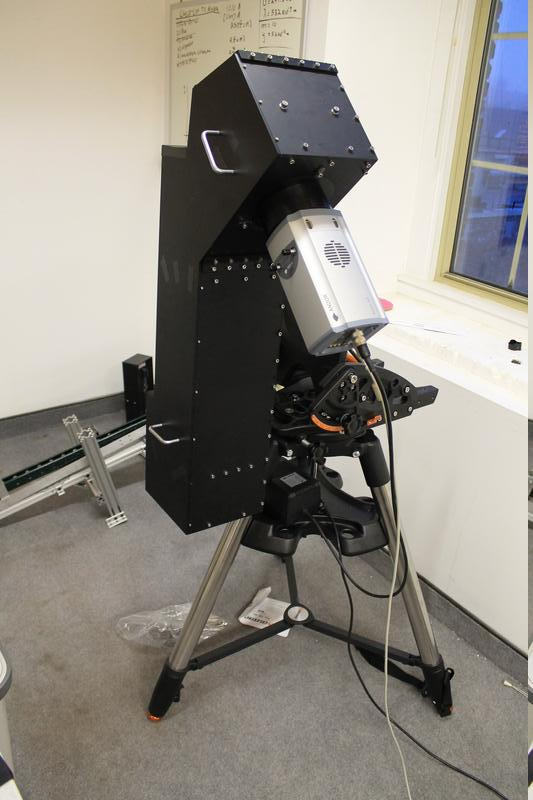
\includegraphics[width=20pc]{Hitmis_tripod_mount.JPG}
	\caption{A: Sample raw image from HiT\&MIS at 22:30 PM LT on June 22, 2015 with 60 s exposure. Overlaid lines are the ray trace estimate of the line center locations of the emission features. B: Photometrically calibrated, background-subtracted 630.0 nm spectrum extracted from the region highlighted in A. C: Average spectrum obtained by integrating over 
		over the entire zenith angle range (y-axis in B) covered by HiT\&MIS.}
	\label{fig:raw}
\end{figure}
%%%%
\begin{figure}[hp]
	\centering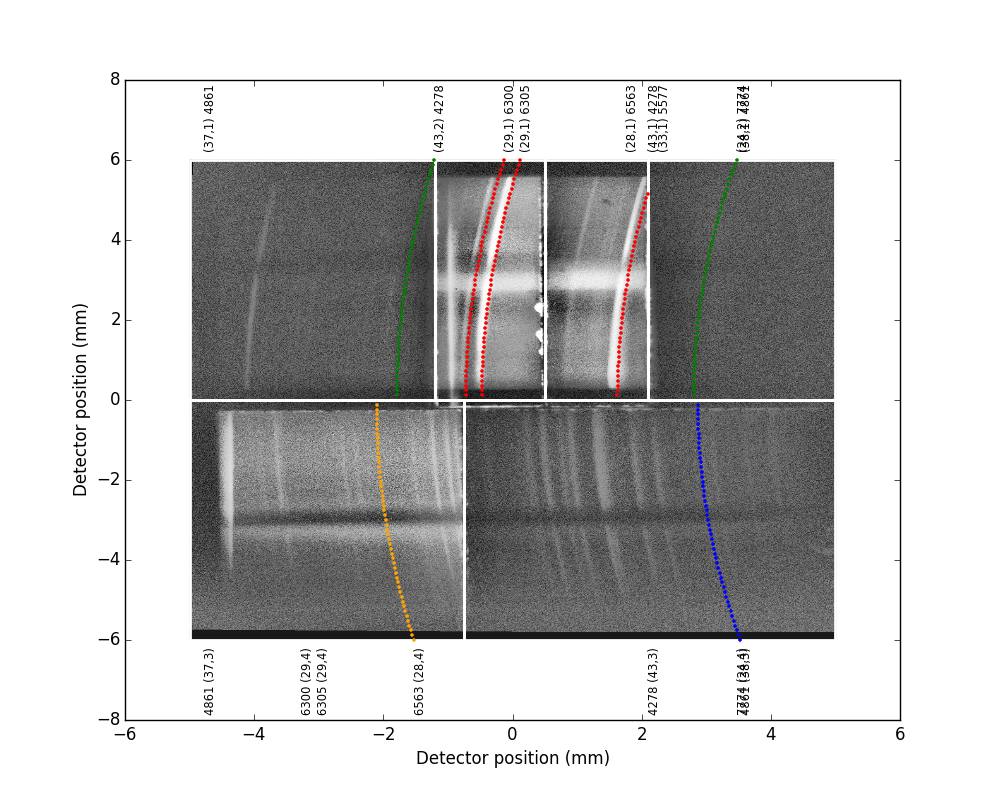
\includegraphics[width=30pc]{hitmis_nighttime.png}
    \centering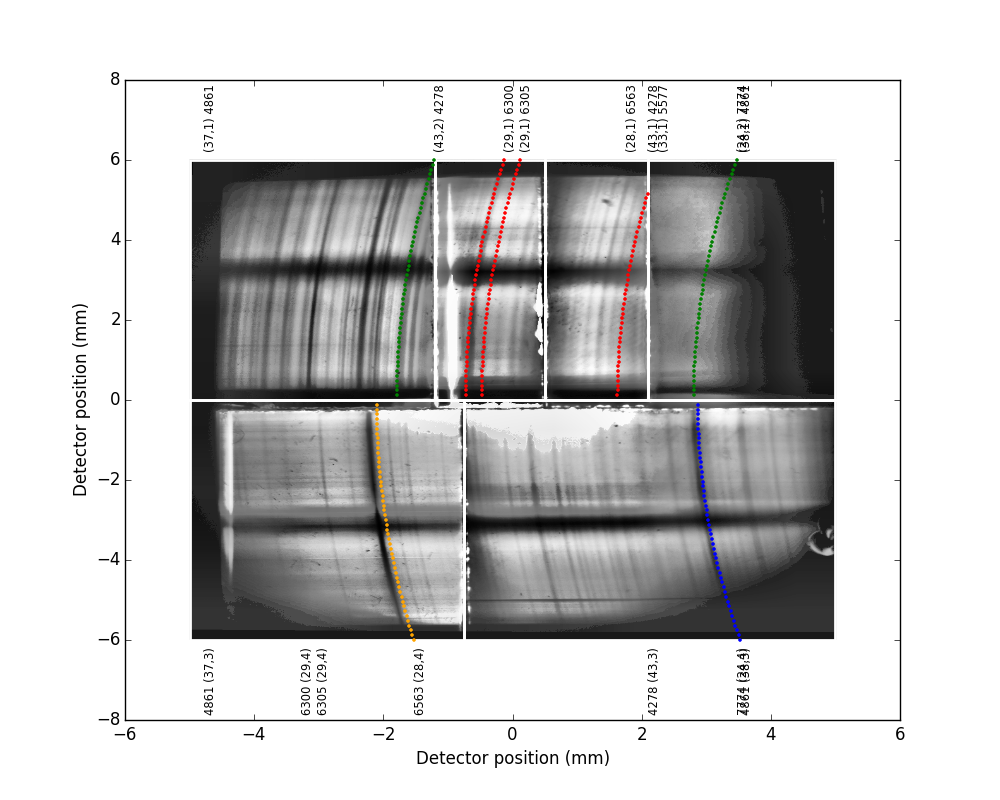
\includegraphics[width=30pc]{hitmis_daytime.png}
	\caption{A: Sample raw image from HiT\&MIS at 22:30 PM LT on June 22, 2015 with 60 s exposure. Overlaid lines are the ray trace estimate of the line center locations of the emission features. B: Photometrically calibrated, background-subtracted 630.0 nm spectrum extracted from the region highlighted in A. C: Average spectrum obtained by integrating over 
		over the entire zenith angle range (y-axis in B) covered by HiT\&MIS.}
	\label{fig:raw}
\end{figure}
